%++++++++++++++++++++++++++++++++++++++++
% Don't modify this section unless you know what you're doing!
\documentclass[letterpaper,10pt]{article}
\usepackage{tabularx} % extra features for tabular environment
\usepackage{amsmath}  % improve math presentation
\usepackage{graphicx} % takes care of graphic including machinery
\usepackage[margin=1in,letterpaper]{geometry} % decreases margins
\usepackage{cite} % takes care of citations
\usepackage[final]{hyperref} % adds hyper links inside the generated pdf file
\hypersetup{
	colorlinks=true,       % false: boxed links; true: colored links
	linkcolor=blue,        % color of internal links
	citecolor=blue,        % color of links to bibliography
	filecolor=magenta,     % color of file links
	urlcolor=blue         
}
%++++++++++++++++++++++++++++++++++++++++


\begin{document}

\title{Report for COMP90025}
\author{Zichun Zhu 784145 zichunz, Yijian Zhang 806676 yijianz }
\date{\today}
\maketitle

\section{Introduction}
The report is aim at counting the number of points in the Mandelbrot Set. The program reads a set of numbers of regions from the command line and output the number of points within the Mandelbrot Set for each region. The hybrid method containing both MPI and OpenMP is used to deal with the task.

\section{Background}
Mandelbrot Set: a collection of points that make up with fractals on a complex plane. The set can be defined as a function does not diverge when iterates from z=0, and the remains are bounded in a specific value. The iteration is shown as follows, c is a complex number.

\section{Methodology}
\subsection{Naive algorithm}
The serial implementation for calculating Mandelbrot Set is generating several points according to the input, and the code will perform an iterative calculation at each point that determine whether the point escape the set. The iteration times which should be big enough also comes from command line, then if the point does not escape, it is considered to be in the Mandelbrot Set. The code iterates over each point, if the point escapes it breaks out of the loop and writes ‘0’ otherwise writes ’1’.

\subsection{Optimization}
First of all, we optimize the algorithm in a mathematical aspect. Including cardioid/bulb checking, periodicity checking, and symmetry checking.

\subsubsection{Cardioid/bulb checking}
It is possible to check whether the incoming point is in the field of cardioid or not. The property of Mandelbrot set shows the set within cardioid region are continuous. We could easily put the x and y into equation .. to check. If the equations are valid , then the point is in the cardioid region, otherwise it is not.

\subsubsection{Periodicity checking}
The repeating z could be occured during iteration. The periodicity checking prevent this happen. However, such checking requires remembering all points have been calculated, so a trade-off is that only remember  the last point it calculated, and if it appear again, the it must in the set.

\subsubsection{Symmetry checking}
Symmetry behavious is one of Mandelbort set’s natures. The set is symmetrical around the real axis. So we could only check one side of the set if which has a adjusted complex number in the set.

\subsubsection{Parallization}
Our implementation for parallelization is based on the serial version. It is noticed that the part of generating points consists of nested ‘for’ loops, which takes a large time when executing, thus it is necessary to parallelize this part using multiple threads. Collapse directive from OpenMP is efficient here that reduce the granularity for work done by each thread, which is benefit for load balancing. Then atomic directive is used to lock each ‘count’ number from confliction. MPI is also initialed before scanning the input so that multiple processes can be used to speed up the code. In addition, after finish counting the points in each process, using MPI Reduce on all process so that each node contributes the number of points, the combining of the points is placed in one process. 

\section{Result}
When the sample is 100 in each dimension the speedup is 0.18/0.24 = 0.75, while the speedup is up to 0.18/0.24 = 71.63 when the sample is 2000. The efficiency is 70.27/(0.981*12) = 5.97 when the sample is 2000, which is the benefit between naive sequential algorithm and the optimal parallel algorithm. If we only consider the benefit from parallelization, the efficiency between optimal sequential algorithm and optimal parallel algorithm equals 20.949/(0.981*12) = 1.78. The efficiency is in the O(1) and we has $\theta(T(2000)/log_c(n))$ processors, so the parallel algorithm could be seems as optimal.
\begin{figure}
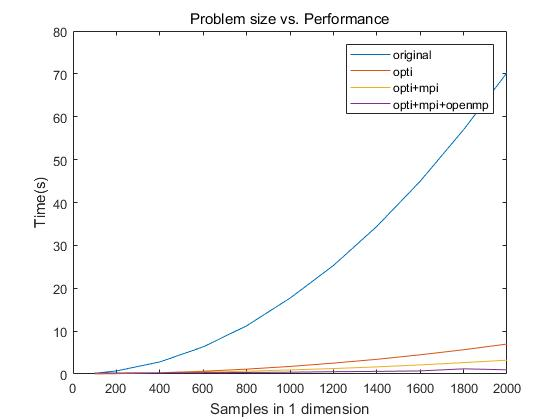
\includegraphics[scale=0.8]{untitled}
\end{figure}

\section{Conclusion}
The hybrid programming using both OpenMP and MPI are useful tools for dealing with the task, it increases the speed of code efficiently, although some overheads are inevitable such as the overhead of creating the thread and process, communication cost between processes. When the calculation get larger enough, the efficient of using parallel method is much better than serial method.
\end{document}
